\chapter{GraphQA}
\label{chap:graphqa}

As stated in the analysis (see chapter \ref{chap:analysis}), GraphQA planned to be a straight forward approach for improving the CONVEX \autocite{paper:convex} prototype on Q0. As a second step, the project would aim toward \gls{nl} generated answers based on the Sub-Knowledge Graphs. As this chapter goes, we could not go as planned during the analysis (see Chapter \ref{chap:analysis}) due to CONVEX complications encountered. However, to our relief, we could bounce back and produce original work. Our final approach started with the naive solution proposed during the analysis (see Chapter \ref{analysis:naive}) and combined it with exciting features we particularly thought meaningful from our analytical brainstorming (see Chapter \ref{analysis:rescoping}). Indeed, in addition to our well defined Multi-Turn Conversations, \gls{mh}, and \gls{wikidata} \gls{kb} Sub-Knowledge Graphs scoped features, we are exploring a \gls{gl} approach by orchestrating various specialized \gls{nlp} models as a global \gls{zero-shot} learning approach for \gls{nl} \gls{qa} chatbots. Finally, we keep the same evaluation settings, as stated in the analysis (see Chapter \ref{analysis:benchmarking}), including the ability for GraphQA to works on top of other \gls{qa} systems.

\section{GraphQA Architecture}
We aim at highlighting in this section the High-Level Architecture evolution from the initial analysis-based scope to our current architecture.

\subsection{Initial Architecture}
\label{graphqa:initial}
As represented in Figure \ref{fig:fig_high_level_convex_architecture_graphqa}, the initial approach for GraphQA was to enhance the CONVEX architecture for the Q0 question (see Chapter \ref{analysis:convexq0}), and then plug a \gls{nl} generator for answers. Finally, the second step was the upgrade of additional CONVEX modules and suggest new use cases to the project, such as a News extension.

\begin{figure}
    \centering
    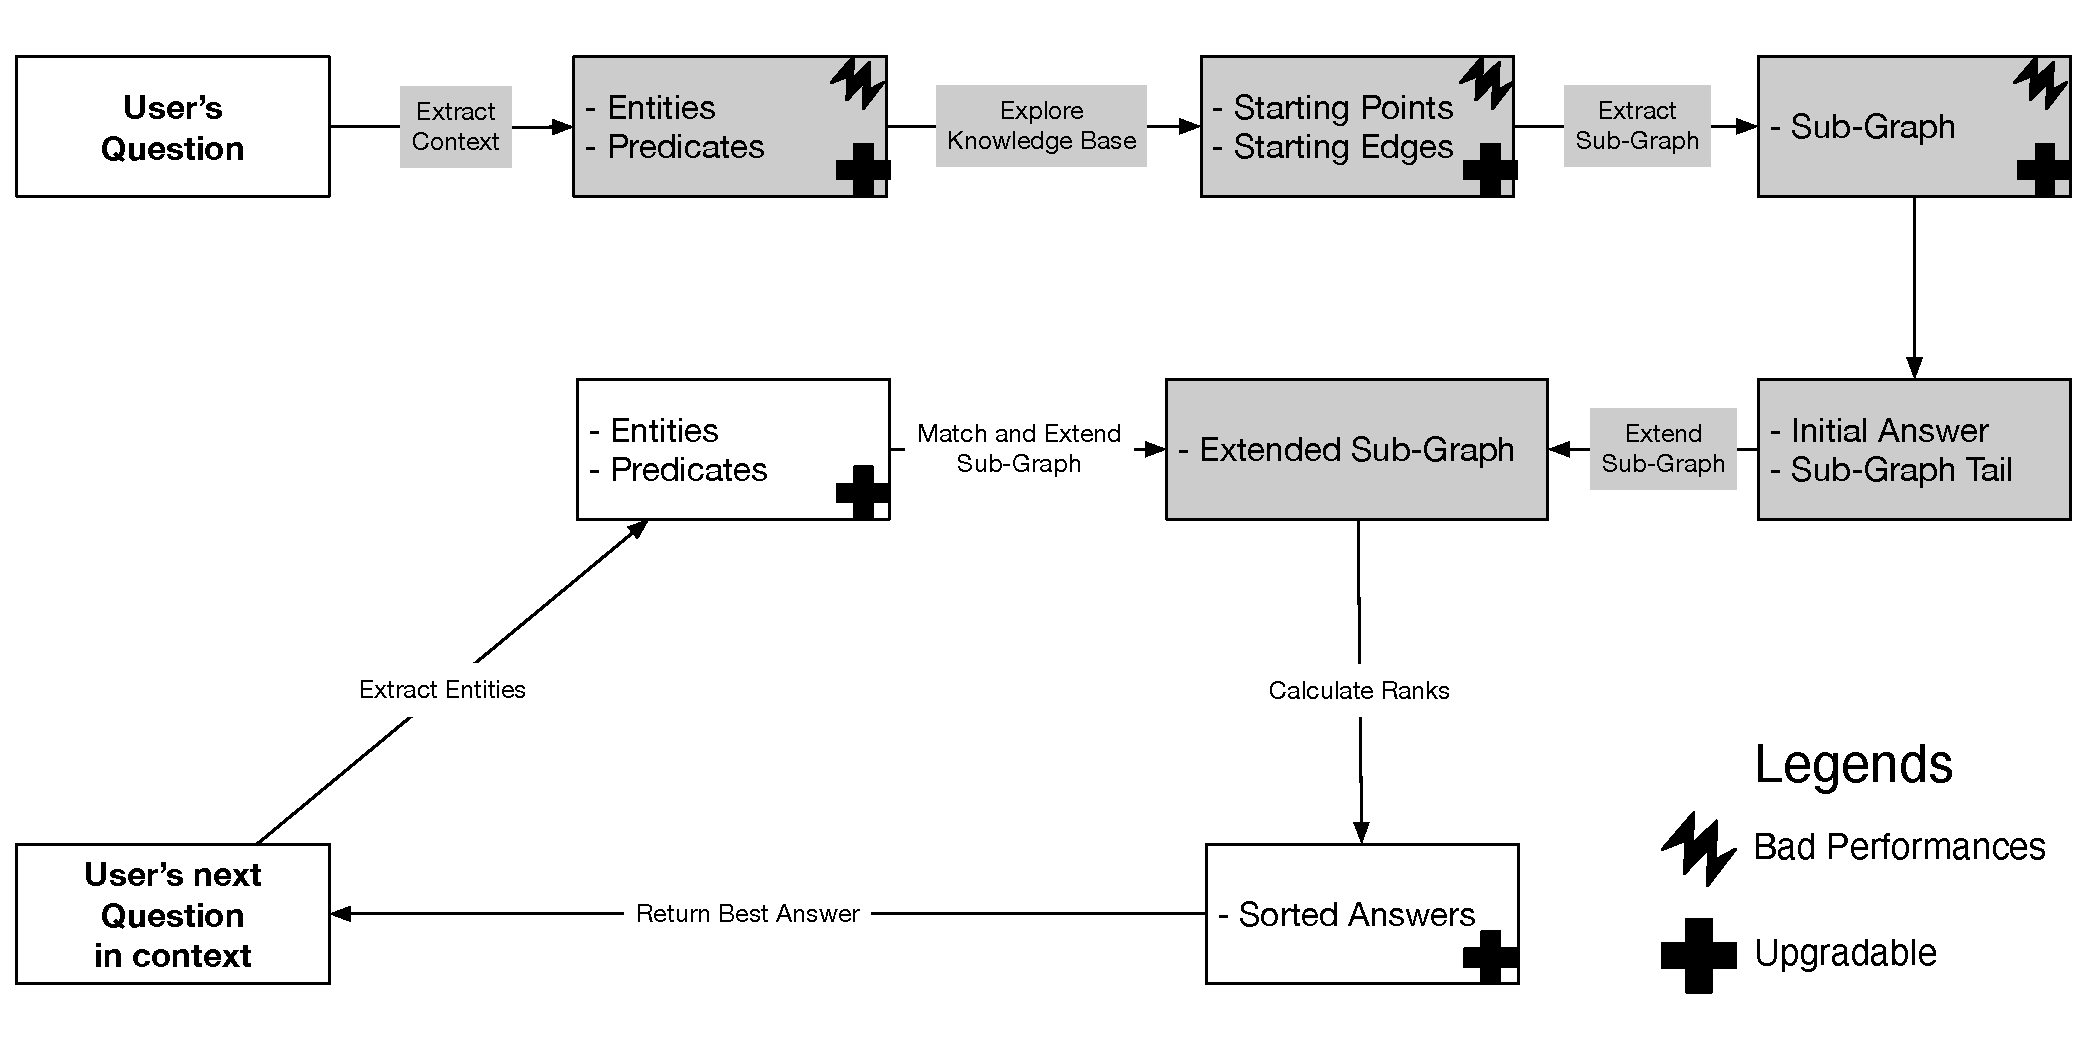
\includegraphics[width=\textwidth,keepaspectratio=true]{fig_high_level_convex_architecture_graphqa}
    \caption{Illustrative representation of the initial high level GraphQA architecture improving CONVEX. In grey, the architecture parts for GraphQA to rebuild.}
    \label{fig:fig_high_level_convex_architecture_graphqa}
\end{figure}



\subsection{Current Architecture}
Our architecture, as represented on Figure \ref{fig:fig_high_level_graphqa_architecture}, results from three major incrementations. It is, at first sight, heavier than the initial CONVEX-based architecture (see previous Section \ref{graphqa:initial}); however, its modular and generic design handles contextual graphs with an overall improvement toward the initial architecture as planned in the analysis. Indeed, as we built the project from the ground-up, we focused on the must-have features and pre-designed anchor points for the nice-to-have features as described in the final scope from our analysis (see chapter \ref{analysis:finalscope}). Additionally, as we aimed at a generic approach via modular orchestration, our \gls{qa} chatbot is by its architecture and design, extensible to further modules by either improve, replace or add new \gls{nlp} tasks.


\begin{figure}
    \centering
    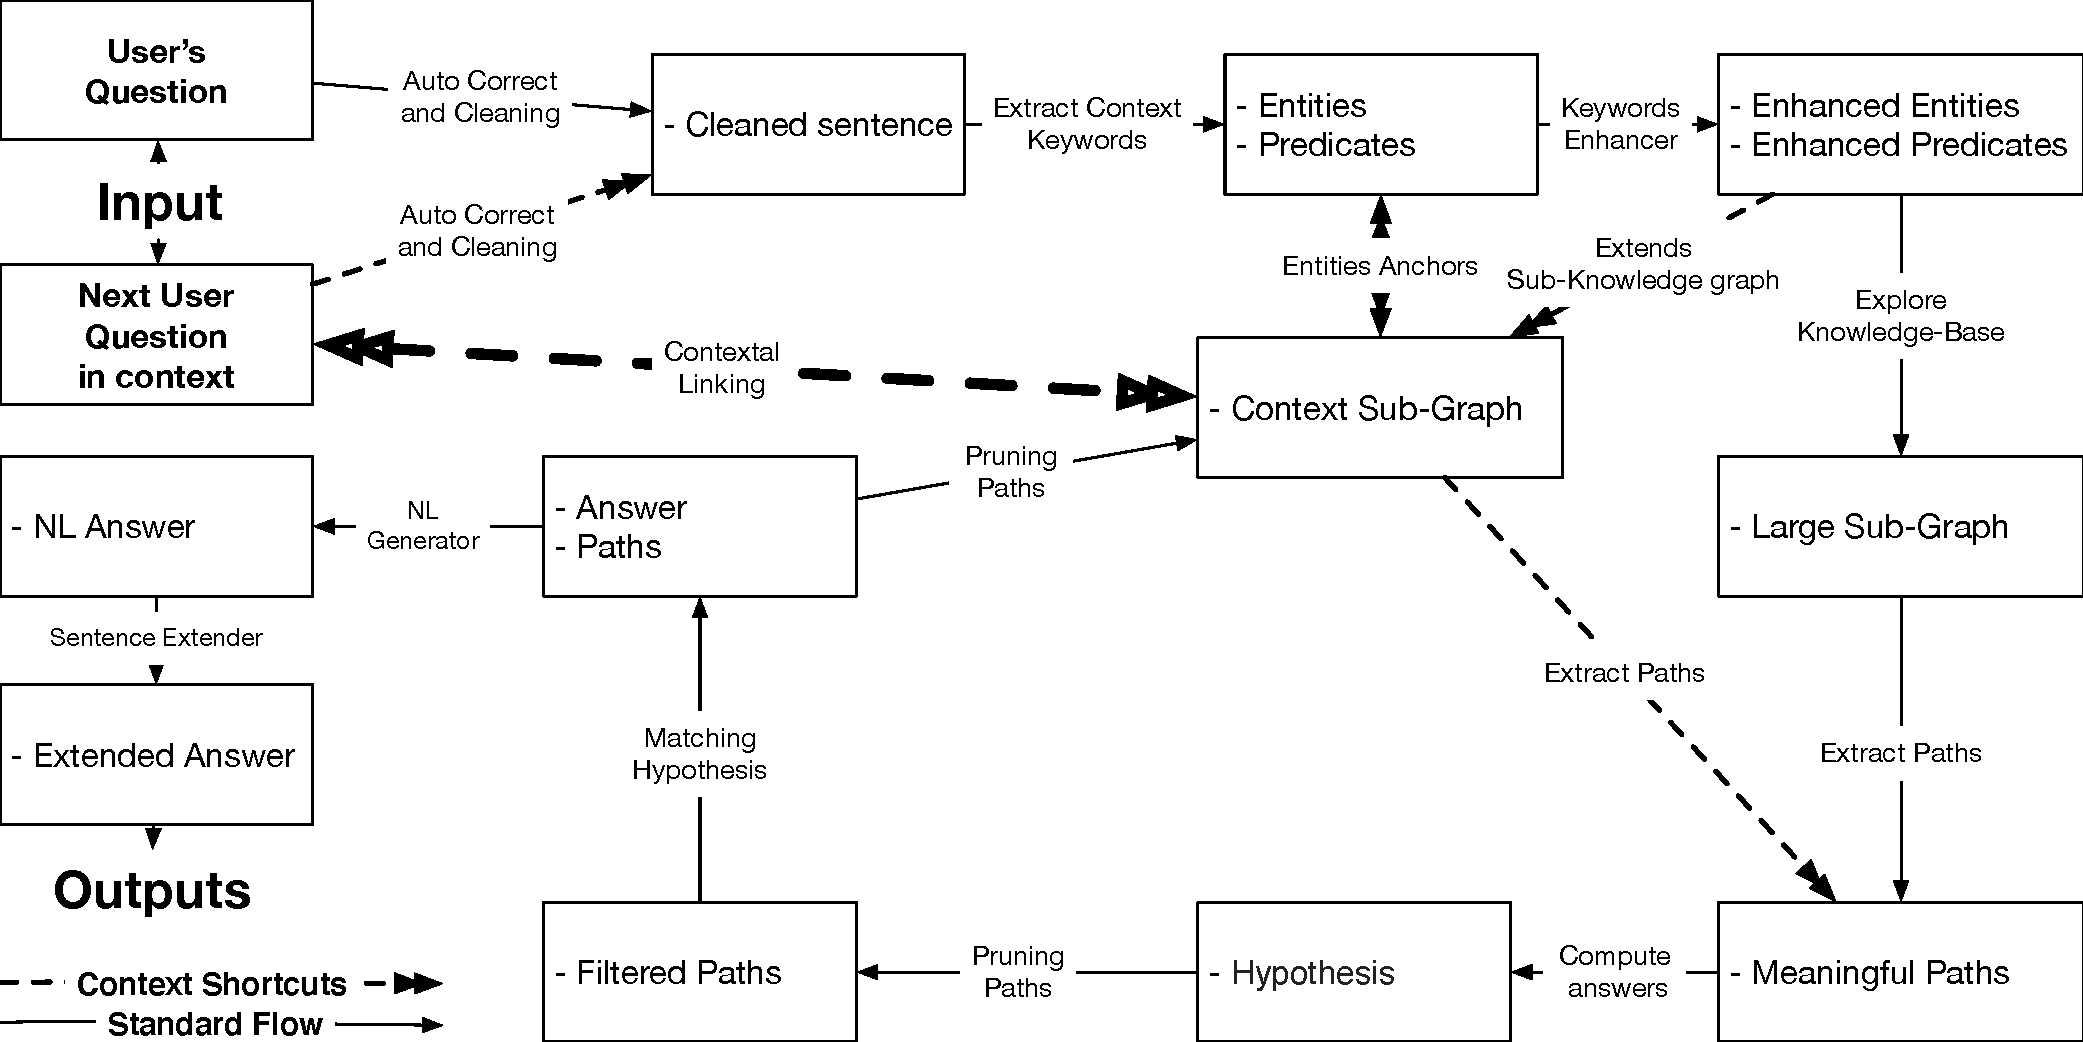
\includegraphics[width=\textwidth,keepaspectratio=true]{fig_high_level_graphqa_architecture}
    \caption{Illustrative representation of current high level GraphQA architecture. Double arrows indicates that the flow is related to context.}
    \label{fig:fig_high_level_graphqa_architecture}
\end{figure}

\subsection{Question Answering Pipeline}
In more details, we present on Figure \ref{fig:fig_graphqa_models_pipeline} our grounded tasks approach, implying a \gls{zero-shot} learning \gls{qa} system, as it doesn't not require any training examples to answer questions.

\begin{figure}
    \centering
    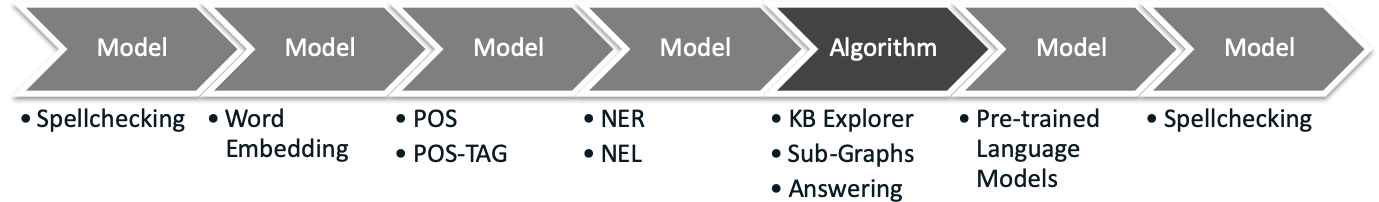
\includegraphics[width=\textwidth,keepaspectratio=true]{fig_graphqa_models_pipeline}
    \caption{Illustrative representation of GraphQA multi-models pipeline.}
    \label{fig:fig_graphqa_models_pipeline}
\end{figure}

\subsection{Dialogue Flow}
To illustrate in more details GraphQA Dialogue flow, Figure \ref{fig:fig_graphqa_dialogue_pipeline} presents our \gls{nl} answering approach for multi-turns conversations.

\begin{figure}
    \centering
    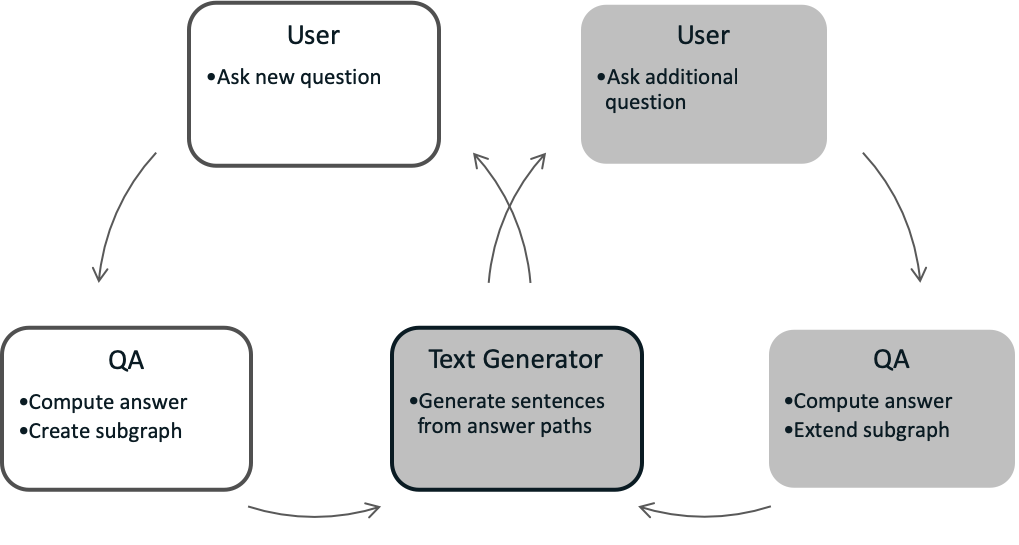
\includegraphics[width=\textwidth,keepaspectratio=true]{fig_graphqa_dialogue_pipeline}
    \caption{Illustrative representation of current GraphQA dialogue pipeline.}
    \label{fig:fig_graphqa_dialogue_pipeline}
\end{figure}

\section{Iteration 0}
The initial GraphQA version was CONVEX-based as we originally scoped to extend CONVEX features (see our previous sections \ref{graphqa:initial}). As we dove into the CONVEX implementation, we came across reproducibility issues and unexpected behaviors. After multiple contacts with the authors, we concluded that our interpretation of their paper was not as they intended to. Indeed, what we believed to be features, were from their point of view made-up feature for motivational purposes, which sadly deeply impacted our \gls{sota} analysis. However, during the initial phase, we understood the tools they built, giving us a head start for our architecture. Indeed, tools such as loading the \gls{wikidata} \gls{kb} and fetching \gls{spo} statements were reusable out-of-the-box. Optimizations such the HDT \autocite{website:hdt} and NetworkX \autocite{paper:SciPyProceedings_11} python libraries were a useful as starting points. 

\section{Major Iteration 1}
\label{graphqa:graphqa1}
Based on the toolset extracted version 0 from the CONVEX-based extender, GraphQA V1 is composed of the features listed below. During the iteration, we saw the opportunity to contribute to the \gls{nlp} field by building a recent version of the \gls{wikidata} \gls{kb} optimized HDT \autocite{website:hdt} format, as the latest dates from September 2018. Sadly, we were not able to generate an HDF dataset from the latest version of \gls{wikidata} \gls{kb} as we didn't have the required ram at our disposal to complete the task (about 240GB for 7.9 Million tuples).

\subsection{Library-based Features}
\label{graphqa:libraries1}
We are listing used libraries in the next section (see Section \ref{graphqa:techno}). Note that we may, in some cases, slightly enhance the basic library features, but we are keeping their main purpose intact.

\begin{itemize}
    \setlength\itemsep{0em}
    \item Retrieving statements from the \gls{wikidata} \gls{kb} via CONVEX
    \item \gls{nel} labels from the \gls{wikidata} \gls{kb} via CONVEX
    \item Document/Span/Word Embeddings via Spacy and GloVe
    \item Tokenization via Spacy
    \item \gls{pos} and \gls{pos-tag} via Spacy
    \item \gls{ner} for common word such as towns, countries, or famous people via Spacy
    \item Extract composed entities via Spacy
    \item Extract nested word groups within sentences via Spacy
    \item Build and explore sub-graphs via NetworkX
\end{itemize}

\subsection{Custom Features}
\label{graphqa:custom1}
The following features were designed with modularity in mind, as stated in the earlier sections. We describe them once here, but they are used in next versions. (See their algorithm subsections).

\subsubsection{Wikidata fine-tuned \gls{ner}}
Spacy's \gls{ner} is particularly impressive out-of-the-box; however, we found the need in the scope of the project to fine-tune Spacy's \gls{ner} model to help it identify Wikidata and Wikipedia pages names.

\subsubsection{Wikidata \gls{nel} training}
Spacy's provides training tools for additional models and includes them natively into its pipeline. We used the opportunity to build a \gls{nel} model linking our fine-tuned \gls{ner} model to also be able to linked the recognised pages to \gls{wikidata} \gls{kb} identifiers.

\subsubsection{Extract themes} 
The entities we call Themes are the most meaning words in a question; they define the initial anchor point to our \gls{qa} system. They have a stronger impact than keywords, as their purpose is to define the question in a meaningful manner.

To extract the question themes, we initially perform an entity check via Spacy's \gls{ner} on the sentence. 

To enhanced the \gls{ner} results, we extract nested word groups within sentences via Spacy's Document Embedding property \textbf{noun\_chunks}, then pass a \gls{ner} on the detected composites.

Additionally, we format the sentences into its Capitalised, Lowercased, Lemmatised, and Determinants-free forms, then apply Spacy's \textbf{noun\_chunks} property to altered sentences and pass a final \gls{ner} on the detected composites.

Note that the detected composites are the themes in our case.

\subsubsection{Enhance themes} 
During the theme extraction process, not all the words in the sentences are used as they have no meaning for our \gls{ner} model. In this module, we give a second chance to the trashed words by trying to match them to \gls{wikidata} entities by exploring the \gls{kb}.

To do so, we apply a similar technique than for theme extraction by formatting the word in their Capitalised, Lowercased, Lemmatised, and Determinants-free in its forms. We combine the words into multi-sized combination tuples then perform a lookup into the \gls{kb} to find a matching identity.

\subsubsection{Extract predicates} 
Often, questions are using inductive nouns or adjectives for predicates, making the naive approach of matching verbs to predicate not efficient. Our solution is to query the \gls{kb} with each word and evaluate the result as predicated. Additionally, we query \gls{wikidata} online with the specific type defining predicates, which often provides additional entities to our initial local query. Note that we initially built GraphQA intending to work in standalone without an internet connection, which makes the web querying sensible to our initial intention, but not against the project scope.

\subsubsection{Extract sentence focused parts} 
The module extracts word syntactically focused by the qualifier, such as who, where, or when. We use those words as initial answer anchors as, in most cases, is it possible to replace this word with the answer, and it converts the question into a descriptive sentence.

\subsubsection{Extract question keywords}
This module aims at capturing the relevant keywords from the question. It categorizes the keywords in three categories, the themes driven keywords, enhanced themes drive keywords, and predicates related to the focused parts. To do so, it uses similar techniques to the \gls{attention} by exploiting the extract word properties by Spacy's Document Embedding model, and the entities present in the sub-knowledge graph.

\subsubsection{Extract keyword related paths}
Based on dynamic thresholds, this module uses previously extracted keywords to extract paths from the raw sub-knowledge graph.

\subsubsection{Filter extracted paths}
The module parses the extract keyword paths to fix malformed \gls{spo} chains by extending further the path and finishes by removing duplicates and sublists.

\subsubsection{Compute answer hypothesizes}
The process consists of rebuilding the question in its descriptive form with \gls{spo} extractions from each filtered path. The final score combines the computed score for each word with an overall rating for each path. The scores are defined either with positive or negative values depending on the evaluated tasks such are word proximities.

\subsubsection{Build the sub-knowledge graph}
Based on the extracted themes, enhanced themes, and predicates, this module explores the \gls{wikidata} \gls{kb} for statements, uses the extracted themes as subject and extracted predicates as predicates and adds matching statements into an empty NetworkX graph.


\subsection{Algorithm}
Here is enumerated the overall process to compute the answer from a question.

\begin{enumerate}
    \setlength\itemsep{0em}
    \item Builds a Document Embedding of the question
    \item Extracts the themes
    \item Extracts the enhanced themes
    \item Extracts the predicates
    \item Extracts the question focused parts
    \item Builds a sub-knowledge graph
    \item Rebuilds the graphs with a higher deepness if it contains too many elements
    \item Extracts the question keywords
    \item Extracts the question-related paths from the sub-knowledge
    \item Filters the extracted paths
    \item Computes and sort hypothesizes
    \item Extracts the paths containing the best hypothesis as the first or last element
\end{enumerate}

\subsection{Major Iteration 2}
\label{graphqa:graphqa2}
In addition to some computational parallelization, tweaks, and optimizations, the second version of GraphQA aims to provide a wiser answer by not trusting the initial best hypothesis score but instead considering all the hypotheses by additionally scoring the matching for each hypothesis within the question itself. We added global banned entities such as linking ids to other \gls{kb}. Finally, the algorithm can handle various computational decisions via predefined thresholds dynamically.

\subsection{Library-based Features}
\label{graphqa:libraries2}
We hereby list only the additional features to the first version (see subsection \ref{graphqa:libraries1}). See Section \ref{graphqa:techno} for the libraries listing.

\begin{itemize}
    \setlength\itemsep{0em}
    \item Auto correcting the questions from the user via DeepCorrect
    \item Replacing recognised names from Wikipedia \gls{ner} within the question via DeepCorrect
\end{itemize}

\subsection{Custom Features}
We hereby list additional and modified features to the first version (see subsection \ref{graphqa:custom1})

\subsubsection{Compute answer hypothesizes by handling types}
The second iteration of this module uses word embedding similarities for its scoring tasks; additionally, it now has the notions of Locations, Persons, Dates, Causes, Quantities, and Selective questions to refine the scoring to the answer types. Finally, we enhanced the scoring formula to handle the overall path score while computing the individual \gls{spo} scores.

\subsubsection{Evaluate hypothesizes}
This module calculates a score for each hypothesis by replacing the hypothesis with the focus part within the question and comparing the new descriptive sentence to the original question. Additionally, it explores the \gls{kb} to reconstruct the original path by giving a higher weight to qualifiers, and gives a score based on the success of the task.

\subsubsection{Answer paths extractor}
Use the fact that we can trust the hypothesizes evaluator to return the best-fitting answer to the question, we enhanced the answer path extractor also to include paths where the answer is not in the first of the last place.

\subsection{Algorithm}
Here is enumerated the overall process to compute the answer from a question. In bold are highlighted the new tasks.

\begin{enumerate}
    \setlength\itemsep{0em}
    \item \textbf{Removes unsupported characters from the question}
    \item \textbf{Autocorrects the question and replaces with Wikipedia names via \gls{ner}}
    \item Builds a Document Embedding of the question
    \item Extracts the themes
    \item Extracts the enhanced themes
    \item Extracts the predicates
    \item Extracts the question focused parts
    \item Builds a sub-knowledge graph
    \item Rebuilds the graphs with a higher deepness if it contains too many elements
    \item \textbf{Rebuilds the graphs with a lower deepness if it does not contain a minimum of elements}
    \item Extracts the question keywords
    \item Extracts the question-related paths from the sub-knowledge
    \item Filters the extracted paths
    \item Computes and sorts hypothesizes
    \item \textbf{Evaluates and sorts the hypothesizes}
    \item \textbf{Extracts the paths containing the best hypothesis}
\end{enumerate}


\section{Major Iteration 3}
\label{graphqa:graphqa3}
In addition to now handle multi-turns conversations within a context sub-graph, GraphQA is completely parallelized, which improves the overall answering speed by 50\%, but does not solve the speed impact of computation (see the results Chapter \ref{chap:results}). Numerous tweaks have taken place and made the overall answering better compared to the previous iteration. Finally, GraphQA in the current state returns answers in \gls{nl}, with the option to extend them with \gls{kb} and random facts.

\subsection{Library-based Features}
We hereby list only the additional features to the second version (see subsection \ref{graphqa:libraries2}). See Section \ref{graphqa:techno} for the libraries listing.

\begin{itemize}
    \setlength\itemsep{0em}
    \item Use of BERT-large pre-trained language model via Huggingface
    \item Use of GPT-2-XL pre-trained generative language model via Huggingface
\end{itemize}

\subsection{Custom Features}
We hereby list additional and modified features to the first version (see subsection \ref{graphqa:custom1})

\subsection{Sub-Knowledge Graph optimnizations}
We enhanced the initial sub-knowledge graph extractor by additionally filtering clusters and removing clusters unrelated to the questions.

\subsection{Binary answers}
This module handles binary questions by exploring the sub-knowledge graph to detect the presence of the focused part.

\subsubsection{Context holding in sub-graphs}
We prune the sub-knowledge graph from clusters entities to the computed answer. We call the pruned sub-knowledge graph Context Graphs, as they only hold the context to the question and previous answer.

\subsubsection{Multi-turn conversations}
In addition to handling context graphs during \gls{qa}, by using the entities already present in the context graph to drive the \gls{kb} exploration and replace pronouns in the new question, the module keeps track of the previous direct questions and weights the keywords to it.

\subsection{\gls{nl} answers}
Until the second version, we returned the fact answer and the best paths from the answer. This module uses the masking feature from \gls{bert} \autocite{paper:devlin-etal-2019-bert} to fill the gaps between \gls{spo} within the answering paths.

\subsection{Context facts extender}
By default, the \gls{nl} answers computes the returned \gls{spo} based on the question, but it is also possible to manually increase the amount of \gls{spo} to return, which increase the original \gls{nl} answers to additional facts extracted from matched paths.

\subsection{Random facts extender}
For gamification purposes, it is also possible to extend the \gls{nl} answers with generated random facts using \gls{gpt2}.

\subsection{Handling Pre-built graph}
GraphQA can be plugged to any \gls{qa} system, as it only requires a context graph, which can hold from none to any amount of nodes and edges, and optionally keywords from the previous conversation. This feature makes it a nice candidate to give the ability to non-conversational \gls{qa} systems to handle Multi-turn conversations.

\subsection{Algorithm}
Here is enumerated the overall process to compute the answer from a question. In bold are highlighted the new tasks.

\begin{enumerate}
    \setlength\itemsep{0em}
    \item Filters the sentence from unsupported characters
    \item Autocorrects the question and replaces with Wikipedia names via \gls{ner}
    \item \textbf{Handles previous context}
    \item Builds a Document Embedding of the question
    \item Extracts the themes
    \item Extracts the enhanced themes
    \item Extracts the predicates
    \item Extracts the question focused parts
    \item \textbf{Extends previous context graph}
    \item Builds a sub-knowledge graph
    \item Rebuilds the graphs with a higher deepness if it contains too many elements
    \item Rebuilds the graphs with a lower deepness if it does not contain a minimum of elements
    \item \textbf{Answers binary questions based on the graph}
    \item Extracts the question keywords
    \item Extracts the question-related paths from the sub-knowledge
    \item Filters the extracted paths
    \item Computes and sorts hypothesizes
    \item Evaluates and sorts the hypothesizes
    \item Extracts the paths containing the best hypothesis as the first element
    \item \textbf{Extracts context graph from sub-knowledge graph}
    \item \textbf{Builds a \gls{nl} answer}
    \item \textbf{Extends the \gls{nl} answer with context graph}
    \item \textbf{Extends the \gls{nl} answer with random facts}
\end{enumerate}


\section{Technologies}
\label{graphqa:techno}
The following are the technologies used by GraphQA.

\paragraph{HDT}
\autocite{website:hdt} It is a query compression format for linked data; it compresses the RDF database and loads its index into the RAM for querying. 

\paragraph{Spacy}
\autocite{paper:spacy2} It is an impressive framework used in the industry for its multiples \gls{nlp} tools, pre-builts models and easy to use fine-tuning pipelines. It allows handles Document Embedding, \gls{we} via GloVe \autocite{paper:glove}, \gls{ner} \gls{nel}, \gls{pos}, \gls{pos-tag}, Tokenization, and much more. On a side note, we used the version 2 released in 2019. 

\paragraph{DeepCorrect}
\autocite{website:deepcorrect-github} It is a project exploring the \gls{dl} for text and punctuation correction with a pre-trained model on Wikipedia.

\paragraph{NetworkX}
\autocite{paper:SciPyProceedings_11} It is a Python package used for the creation and manipulation of graphs.

\paragraph{Huggingface}
\autocite{paper:2019arXiv191003771W} It is a startup focusing on \gls{nlp} tools, in particular \glspl{transformer}. They provide frameworks to use pre-trained language model out-of-the-box, making them popular in the \gls{nlp} field and the industry.

\section{Dev Benchmarking Questions}
For each GraphQA version, we used the same six development questions to evaluate our work superficially. Additionally, we incrementally increased a pool of questions triggering error while performing benchmarks on the SimpleQuestions and ConvQuestions datasets, which we kept as debugging purposes and tracker for the consistency across our incremental versions.

\subsection{Single-hop Questions}
Here is our two development \gls{sh} questions.
\begin{itemize}
    \setlength\itemsep{0em}
    \item \say{Who is the wife of Barack Obama?}
    \item \say{of what nationality is ken mcgoogan}
\end{itemize}
    

\subsection{Multi-hop Questions}
Following is our two development \gls{mh} questions.
\begin{itemize}
    \setlength\itemsep{0em}
    \item \say{What is the name of the writer of The Secret Garden?}
    \item \say{Which actor voiced the Unicorn in The Last Unicorn?}
\end{itemize}

\subsection{Multi-hop and Multi-Turns Questions}
Following our two development \gls{mh} and multi-turn questions.
\subsubsection{Conversation 1}
\begin{enumerate}
    \setlength\itemsep{0em}
    \item \say{Which actor voiced the Unicorn in The Last Unicorn?}
    \item \say{And Alan Arkin was behind..}
    \item \say{Who did the score?}
    \item \say{So who performed the songs?}
    \item \say{Genre of this band}
    \item \say{By the way, who was the director?}
\end{enumerate}

\subsubsection{Conversation 2}
\begin{enumerate}
    \setlength\itemsep{0em}
    \item \say{Who is the author of the Harry Potter series?}
    \item \say{What was the year of publication for the first book?}
    \item \say{The first book was called what?}
    \item \say{It was set in what country?}
    \item \say{Which book has the highest page count?}
\end{enumerate}


\section{Further Exploration Ideas}
This section provides a non-exhausting list of exploratory ideas for future related studies.

\begin{itemize}
    \setlength\itemsep{0em}
    \item Use a pre-trained language model such as \gls{bert} as word embedding instead of GloVe.
    \item Fine-tune a pretrain language model such as \gls{bert} for \gls{nel}.
    \item Fine-tune a pretrain language model such as \gls{bert} to add a multi-brains approach as slightly mentioned in the analysis \ref{chap:analysis} brainstorming. Where multiple models are answering simultaneously the same question, and reach a consensus for the final answer.
    \item Query \gls{wikidata} online for cross-checking local entities and enhanced themes.
    \item Prebuild context graph for contents such as Articles to increase speed and target the information.
    \item Context graph bridging multiple prebuilt graphs to gather information faster and long-distance context handling
    \item Extend context graphs for user experience personalization by keeping long-term contexts.
\end{itemize}


\section{Interesting Facts}
On a final note, we also wanted to mention a non-exhausting list of problems that occurred during the making of GraphQA that we believe are interesting facts.

\begin{itemize}
    \setlength\itemsep{0em}
    \item The uncompressed version of the latest \gls{wikidata} dump is 500 GB.
    \item Knowledge Bases do not have the same conventions for Subject-Predicate-Object Tuples (SPOs).
    \item Nested Tensorflow sessions are not working as expected when called.
\end{itemize}


